\subsection{The Turing machine $M_\text{binaryunary}$}

This Turing machine, on binary input $w\in \{0,1\}^*$ (least significant bit first) should halt in the accepting state leaving the unary equivalent of this number on the tape. On other words, if the input $w$ represents the number $x\in\mathbb{N}$, the contents of the tape upon halting in the accepting state should be $1^x$. 

The table below shows some examples.

\begin{center}
    \begin{tabular}{l|l}
         tape input, $w$ & tape output \\
         \hline
         $\_$ & $\_$ \\
         $1$ & $1$ \\
         $10$ & $1$ \\
         $01$ & $11$ \\
         $011$ & $111111$
    \end{tabular}
\end{center}


\subsubsection{Description}

\paragraph{High-level description}
Repeatedly, we decrement the binary number by one and append a $\#$ to the end of the tape. Once the binary number is $0$, move each $\#$ to the beginning of the tape, converting each to a $1$.

\paragraph{Implementation-level description}
$M_{\text{binaryunary}}=$
``on input $w \in \{0,1\}^*$:

\begin{enumerate}
    \item Move every tape symbol one to the right and make the leftmost tape symbol to be $\$$. While this is not strictly necessary (and will increase the number of transitions required), this will make the implementation easier. 
    \item Move right until we encounter a $1$. 
        \begin{itemize}
            \item If, in doing so, we encounter a $\_$, instead clear the tape (replace all cells with $\_$) and accept.
            \item If, in doing so, we encounter a $\#$, instead move one cell left and go to step 7.
        \end{itemize}
    \item Write $Y$ to that cell and move right until we encounter $\_$.
    \item Write $\#$ to that cell and move left until we encounter $Y$.
    \item Write $0$ to that cell and move left until we reach $\$$. In doing so, replace each $1$ with $0$, but leave the $0$s as $0$s.
    \item Go to step 2.
    \item Move left (reading $0$s) until either of the following conditions holds:
        \begin{itemize}
            \item we encounter a $1$, in which case we move one right and write $1$ to that cell (on the right); or 
            \item we encounter a $\$$, in which case we write $1$ to the tape and move one cell to the right.
        \end{itemize}
    \item Move right while reading $0$s, until:
    \begin{itemize}
        \item we encounter a $\#$, in which case we write $0$ to the tape, move one left and go to step 7; or
        \item we encounter the end of the tape ($\_$), in which case we move left while reading $0$s and replacing them with $1$, and once we encounter $1$, accept."
    \end{itemize}
\end{enumerate}

\subsubsection{Theoretical analysis of complexity}

\begin{wrapfigure}{r}{0.25\textwidth}
    \centering
    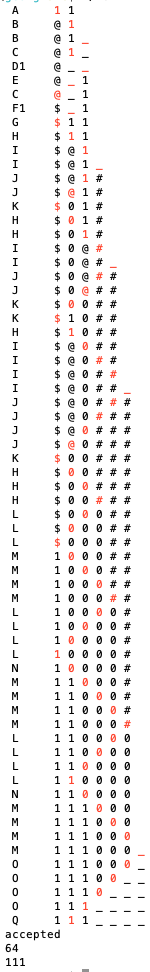
\includegraphics[width=2.5cm]{images/screenshots/binaryunary.png}
    \vspace{-5cm}
\end{wrapfigure}

Clearly, the word $x_n$ that will require the most transitions for a particular $n$ will be of the form $x_n=1^n$, as this will be the largest binary number that can be represented in that space, and as a result, the machine will need to write the most $1$s to the tape.

On input $x_n=1^n$ (as seen in the example screenshot to the right where $n=2$):

\begin{enumerate}
    \item We move to the end of the tape ($n$ transitions). Then we move each symbol one to the right, and set the leftmost symbol to $\$$ ($3n$ transitions).
    \item We move over the binary number, marking the first $1$ we encounter ($n$ transitions). If we do not encounter a 1 until reaching $\#$ or $\_$, go to step 5.
    \item Let $i$ denote the current number of $\#$ characters at the end of the word (initially $i=0$). We need to move past all the $\#$ characters and append an extra $\#$ at the end ($i+1$ transitions).
    \item We move back to the start of the tape, decrementing the binary number by one while doing so ($i+n+1$ transitions). Then, we go to step 2 (this means steps 2-4 will be repeated until $i=2^n-2$).
    \item Write 0 to the current cell and move to the beginning of the tape ($n+1$ transitions).
    \item Write 1 into the current cell and move right until encountering $\#$ ($n+2$ steps).
    \item Write 0 into the current cell and move left until encountering $1$ ($n+2$ steps).
    \item Write 1 into the current cell and move right until encountering $\#$ ($n+3$ steps). Go to step 7 (total of $2^n-2$ repeats). 
    \begin{itemize}
        \item If, instead, we encounter $\_$, move left, writing $\_$ to the tape while reading $\#$ and accept ($n+2$ steps).
    \end{itemize}
\end{enumerate}

Counting the number of transitions in terms of $n$, we obtain
\begin{align*}
    f(n) &=
        n + 3n +
        \sum_{i=0}^{2^n-2}(n + i + 1 + i + n + 1) +
        2(n + 1) + n + 2 \\ &+
        (n + 2 + n + 3)(2^n - 2) + 
        n + 2 \\
    &= (2n + 5)(2^n - 2) + 8n + 6 + \sum_{i=0}^{2^n-2}(2n + 2i + 2) \\
    &= (2n + 5) 2^n + 4n - 4 + \sum_{i=0}^{2^n-2}(2n + 2i + 2) \\
    &= (2n + 5) 2^n + 4n - 4 + \frac{2^n - 1}{2}(2n+2+2n+2(2^n-2) + 2) \\
    &= (2n + 5) 2^n + 4n - 4 + \frac{2^n - 1}{2}(4n + 2(2^n)) \\
    &= (2n + 5) 2^n + 4n - 4 + (2^n - 1)(2n + 2^n) \\
    &= (2^n + 4n + 4) 2^n + 2n - 4 \\
    &= 4^n + n 2^{n+2} + 2^{n+2} + 2n - 4.
\end{align*}

As a result,
$$ M_\text{binaryunary} \in \text{DTIME}(4^n + n 2^{n+2} + 2^{n+2} + 2n - 4), $$
and so its complexity is in the order of $\mathcal{O}(4^n)$.

\subsubsection{Paractical analysis of complexity}

The theoretical results are evident in practical trials. The data collected in \code{data/binaryunary-ones.csv} confirms the findings of $f$ (the values were cross-checked). Furthermore, the plot below shows how this worst-case scenario behaves as a plot of $n$ against the number of transitions made by the machine. Note that the number of steps explodes so quickly that we only plot until $n=16$.

\begin{center}
    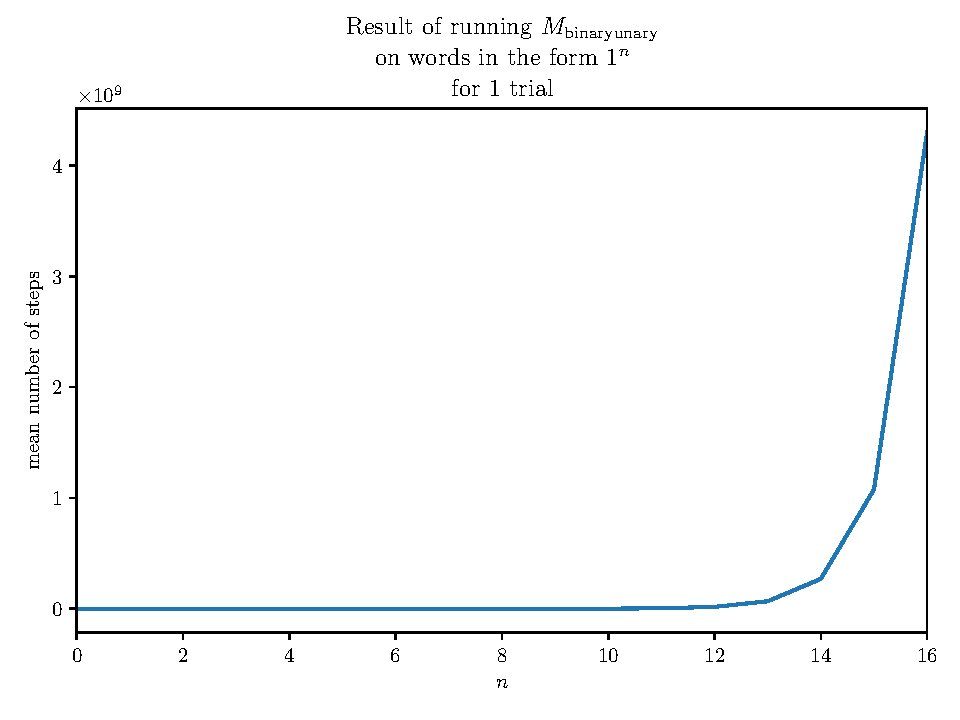
\includegraphics[width=\textwidth]{images/plots/binaryunary-ones.pdf}
\end{center}

Other types of input words were also tested; please refer to the plots in section \ref{plots_binaryunary}, as well as the CSV data in \code{data/binaryunary-*.csv}. 